\graphicspath{{./lab03/Images/}}


\maketitlepage{App Development}{in Android Studio}{Lab 3: Components}
\maketocpage


\section{Activities}
We have already used an activity without going into too much detail what it is. An activity is a single screen unit (usually full screen) with an user interface. So far we have only worked with a single activity but an Android app can have multiple activities. It breaks the app up into section with different purpose and UI. For example, a menu in an email app could be an activity while composing an email might be another, opened from the menu.\\

One activity serves as a luncher activity. It is our starting point when running the app (opposed to a C\texttt{++} main function) and from there on we can start navigating to other activities if any. Every app must have a luncher activity. All activities must be declared in our app's manifest\footnote{Android Studio does this automatically when an activity is created} and the luncher activity is also determined there.\\

Each activity uses a layout file that defines their UI at leat partially (some of it may be done dynamically in Java). In the \texttt{onCreate} function we have been setting the activity's layout with the \texttt{setContentView} method. Activities can share layouts although it serves a limited purpose unless most of the UI is dynamic. We will look at better ways to share UI in Fragments.\\

\subsection{Starting a new Activity}
Lets start by creating a new activity with \menu{File > New > Activity > Empty Activity} and name it \texttt{SecondActivity} and leave the other options as they are. Before proceeding you should inspect your manifest. Add a button to the luncher activity which calls the method \texttt{clicked()} upon being clicked and add some text to the second activity so it differentiates from the other one. Finally add the following method to the luncher activity and run the progam.

\begin{lstlisting}[style=A_Java]
public void clicked(View view) {
    startActivity(new Intent(MainActivity.this, SecondActivity.class));
}	
\end{lstlisting}

The \texttt{startActivity} method takes \texttt{Intent} as a paramter. We will look at that class, its parameters and methods in more detail later but for now, you can think of it as a bridge between two activities. 

\subsection{Lifecycle}
Activities are managed by a stack called the activity stack (or the back stack) and whatever activity is in our foreground is at the top of our stack. During the lifecycle of an activity, it can have various states and the event that brings us to set states have their own callback methods. This lifecycle can be seen in figure \ref{fig:actlife}.

\begin{figure}[H]
\centering
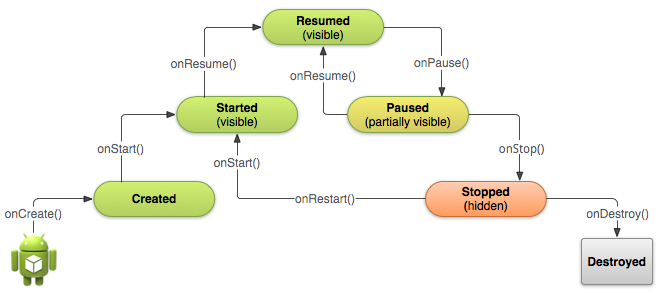
\includegraphics[scale=.5]{activity_state_machine.png}
\caption{The lifecycle of an Activity}
\label{fig:actlife}
\end{figure}

The states are
\begin{itemize}
	\item \textbf{Starting}. In the process of setting up.
	\item \textbf{Running}. In foreground.
	\item \textbf{Paused}. Not in foreground.
	\item \textbf{Stopped}. Inactive but remains in memory.
	\item \textbf{Destroyed}. Shut down and removed from memory.
\end{itemize}

There are multiple callback methods called when moving between states. We have already seen \texttt{onCreate} which is the only one that activities are required to override but there are several others.

\begin{itemize}
	\item \textbf{\texttt{onCreate()}}.\\
    \noindent This callback method is for the event of creating an activity and is called before the activity starts for the first time. It is typically used for initialization as we have been using it already.
	\item \textbf{\texttt{onStart()}}.\\
    \noindent Is called every time the activity starts, after entering the starting state. Here the activity becomes visible and prepares for entering the foreground and becoming interactive. This is where the app initializes the code that maintains the UI of the activity.
	\item \textbf{\texttt{onResume()}}.\\
    \noindent When entering the running state the activity is coming to the foreground and this callback is invoked. Here we should initialize components that are released by \texttt{onPause}, such as animations and camera.
	\item \textbf{\texttt{onPause()}}.\\
    \noindent This method is invoked when you are leaving your activity and it seizes to be in the foreground but is still visible. From there on it can either be resumed later or stopped. Here we must release system resources such as GPS and camera as well as animations but we should not perform long and heavy tasks of cleaning up here.
	\item \textbf{\texttt{onStop()}}.\\
    \noindent After your activity siezes to be visible, this callback is invoked. The \texttt{onPause} method is always called before this one and any large task of releasing resources should happen here. The activity is still in memory at this stage.
	\item \textbf{\texttt{onRestart()}}.\\
    \noindent If the activity goes from being stopped to starting it will invoke the \texttt{onRestart} method.
	\item \textbf{\texttt{onDestroy()}}.\\
    \noindent When you are removing your activity from memory this method is invoked but at what time exactly is unpredictable. To destroy our current activity we can call the \texttt{finish} method.
\end{itemize}

Using \texttt{Log.d} we can use printf debugging with certain tags and filter them with the Android monitor as shown in figure \ref{fig:logfilt}. 

\begin{figure}[H]
\centering
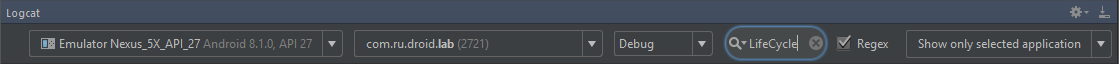
\includegraphics[scale=.7]{log.png}
\caption{Filter logs}
\label{fig:logfilt}
\end{figure}

Using \texttt{Log.d} we can monitor the lifecycle of the two activities found in listings \ref{listing:twoactxml} and \ref{listing:twoactjava}. You should try various scenarios of navigating between the apps as well as rotating the screen and using the Android back button.

\begin{lstlisting}[style=A_XML,caption={Two layouts for two activities},label={listing:twoactxml}]
<?xml version="1.0" encoding="utf-8"?>
<LinearLayout xmlns:android="http://schemas.android.com/apk/res/android"
    xmlns:tools="http://schemas.android.com/tools"
    android:layout_width="match_parent"
    android:layout_height="match_parent"
    android:orientation="vertical"
    android:gravity="center"
    tools:context="com.ru.droid.lab.MainActivity">
    <TextView
        android:layout_width="wrap_content"
        android:layout_height="wrap_content"
        android:text="Activity 1"/> <!-- move to res -->
    <Button
        android:layout_width="wrap_content"
        android:layout_height="wrap_content"
        android:onClick="gotoWithoutFinish"
        android:text="goto 2"/> <!-- move to res -->
    <Button
        android:layout_width="wrap_content"
        android:layout_height="wrap_content"
        android:onClick="gotoAndFinish"
        android:text="goto 2 and finish"/> <!-- move to res -->
</LinearLayout>

<?xml version="1.0" encoding="utf-8"?>
<LinearLayout xmlns:android="http://schemas.android.com/apk/res/android"
    xmlns:tools="http://schemas.android.com/tools"
    android:layout_width="match_parent"
    android:layout_height="match_parent"
    android:orientation="vertical"
    android:gravity="center"
    tools:context="com.ru.droid.lab.SecondActivity">
    <TextView
        android:layout_width="wrap_content"
        android:layout_height="wrap_content"
        android:text="Activity 2"/> <!-- move to res -->
    <Button
        android:layout_width="wrap_content"
        android:layout_height="wrap_content"
        android:onClick="gotoWithoutFinish"
        android:text="goto 1"/> <!-- move to res -->
    <Button
        android:layout_width="wrap_content"
        android:layout_height="wrap_content"
        android:onClick="gotoAndFinish"
        android:text="goto 1 and finish"/> <!-- move to res -->
</LinearLayout>

\end{lstlisting}

\begin{lstlisting}[style=A_Java,caption={Overriding on activity lifecycle callbacks for two activities},label={listing:twoactjava}]
public class MainActivity extends AppCompatActivity {
    @Override
    protected void onCreate(Bundle savedInstanceState) {
        super.onCreate(savedInstanceState);
        setContentView(R.layout.activity_main);
        Log.d("LifeCycle", "Activity 1: onCreate");
    }
    @Override
    protected void onStart() {
        super.onStart();
        Log.d("LifeCycle", "Activity 1: onStart");
    }
    @Override
    protected void onResume() {
        super.onResume();
        Log.d("LifeCycle", "Activity 1: onResume");
    }
    @Override
    protected void onPause() {
        super.onPause();
        Log.d("LifeCycle", "Activity 1: onPause");
    }
    @Override
    protected void onStop() {
        super.onStop();
        Log.d("LifeCycle", "Activity 1: onStop");
    }
    @Override
    protected void onDestroy() {
        super.onDestroy();
        Log.d("LifeCycle", "Activity 1: onDestroy");
    }
    public void gotoWithoutFinish(View view) {
        startActivity(new Intent(MainActivity.this, SecondActivity.class));
    }
    public void gotoAndFinish(View view) {
        startActivity(new Intent(MainActivity.this, SecondActivity.class));
        finish();
    }
}

public class SecondActivity extends AppCompatActivity {
    @Override
    protected void onCreate(Bundle savedInstanceState) {
        super.onCreate(savedInstanceState);
        setContentView(R.layout.activity_second);
        Log.d("LifeCycle", "Activity 2: onCreate");
    }
    @Override
    protected void onStart() {
        super.onStart();
        Log.d("LifeCycle", "Activity 2: onStart");
    }
    @Override
    protected void onResume() {
        super.onResume();
        Log.d("LifeCycle", "Activity 2: onResume");
    }
    @Override
    protected void onPause() {
        super.onPause();
        Log.d("LifeCycle", "Activity 2: onPause");
    }
    @Override
    protected void onStop() {
        super.onStop();
        Log.d("LifeCycle", "Activity 2: onStop");
    }
    @Override
    protected void onDestroy() {
        super.onDestroy();
        Log.d("LifeCycle", "Activity 2: onDestroy");
    }
    public void gotoWithoutFinish(View view) {
        startActivity(new Intent(SecondActivity.this, MainActivity.class));
    }
    public void gotoAndFinish(View view) {
        startActivity(new Intent(SecondActivity.this, MainActivity.class));
        finish();
    }
}
\end{lstlisting}


\subsection{Passing data between activities}




\section{Fragments}
\section{Services}

\section{Assignment}